\chapter{Feature descriptor} \label{sec:feature_descriptor}

For a computer, a picture is represented as a 2-D or 3-D array. To facilitate the classification, feature descriptor extract derived values (the features), calculated to be more informative and invariant to some common picture transformations.

As such, colour is one of the key components of a food item, thus it is widely applied for classification. Colour statistics are commonly used, such as the first and second moment values for different channels. It can be computed for multiple colour representations (RGB, HSV, grey, YCrCb or L*a*b* space).

Another import feature of food is the texturee. Numerous texture descriptors can be used such as Gabor filters or Local Binary Pattern.

\section{Local binary pattern}

% http://www.pyimagesearch.com/2015/12/07/local-binary-patterns-with-python-opencv/

Local binary pattern is a visual descriptor for texture composition of an image, first presented in 2002 in \cite{Ojala2002} (although the concept of LBPs were introduced as early as 1993).

\subsection{Gray-scale LBP}

The figure \ref{fig:lbp_process} represents an example of the LBP in which the LBP code of the centre pixel (in red color and value 20) is used as a local intensity threshold : the neighbour pixels whose intensities are equal or higher than the centre pixel’s are labelled as ”1”; otherwise as ”0”. Then, starting always from the same point, we can transform this binary string to decimal and is used to describe the central pixel. In this example we start at the top-right point and work our way clockwise accumulating the binary string as we go along and obtain the value 24.

\begin{figure}[h]
    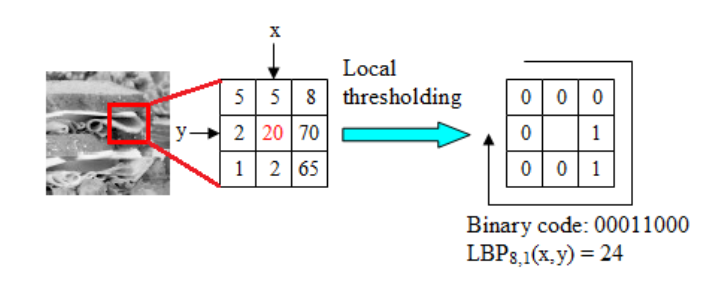
\includegraphics[scale=0.55]{img/lbp}
    \caption{Illustration of the LBP descriptor's process}
    \label{fig:lbp_process}
\end{figure}

Given a pixel $c = (x_c, y_c)$, the value of the $LBP$ code of $c$ is defined as:
$$LBP_{P, R} (x_c, y_c) = \sum_{p = 0}^{P - 1} s (g_p - g_c) 2^p$$
where:
\begin{itemize}
    \item $p$ is a neighbour pixel of $c$ and the distance from $p$ to $c$ does not exceed $R$. Thus, $R$ is the radius of a circle centred in $c$ and $P$ is the numbered of sampled points.
    \item $g_p$ and $g_c$ are the grey values (intensities) of $p$ and $c$
    \item $s(x)$ is the function defined as:
    \begin{equation}
    s(x) =
    \begin{cases}
    1 & \text{if $x \geq 0$}\\
    0 & \text{otherwise} \\
    \end{cases}
    \end{equation}
\end{itemize}

In Fig. \ref{fig:lbp_process}, $R$ and $P$ are 1 and 8 respectively.

The number of histograms bins for $LBP_{P, R}$ is $2^P$.

\subsection{Uniform LBP}

This algorithm has been enhanced to make it rotation invariant. Still in \cite{Ojala2002}, the authors introduce the notion of uniform LBP. A LBP is considered to be uniform if it has at most two bitwise transitions (0 to 1 or 1 to 0 transitions in the binary word). 

For example, the pattern \textit{01000000}  (2 transitions) and \textit{11111110} (1 transition) are both considered to be uniform. For a $LBP_{P, R}$, there is $p + 1$ possible uniforms.

Non-uniform LBP are considered as noise and are assigned the same constant value.

Thus, for uniform LBP, we use the formula:

$$
LBP_{P, R}^{uni} (x_c, y_c) = 
\begin{cases} \displaystyle
\sum_{p = 0}^{P - 1} s (g_p - g_c) 2^p & \text{if uniform} \\
P + 1 & \text{otherwise} \\
\end{cases}
$$

\section{Color descriptor}
\subsection{Color histogram}

HSV space is composed of:
\begin{itemize}
    \item \textbf{Hue} channel: represents the dominant spectral component—colour in its pure form, as in green, red, or yellow
    \item \textbf{Saturation} channel: represents the white added to the pure color (the Hue)
    \item \textbf{Value} channel: represents the brightness of the colour
\end{itemize}

Hue and Saturation corresponds to the chromaticity of the colour. For the joint histogram (2D histogram), the H and S channels are used as value is dependant of the condition where the picture were taken, thus is not interesting. The coordinate system is cylindrical, and is often represented by a six-sided inverted pyramid (see figure \ref{fig:hsv_pyramid}).

\begin{figure}
    \centering
    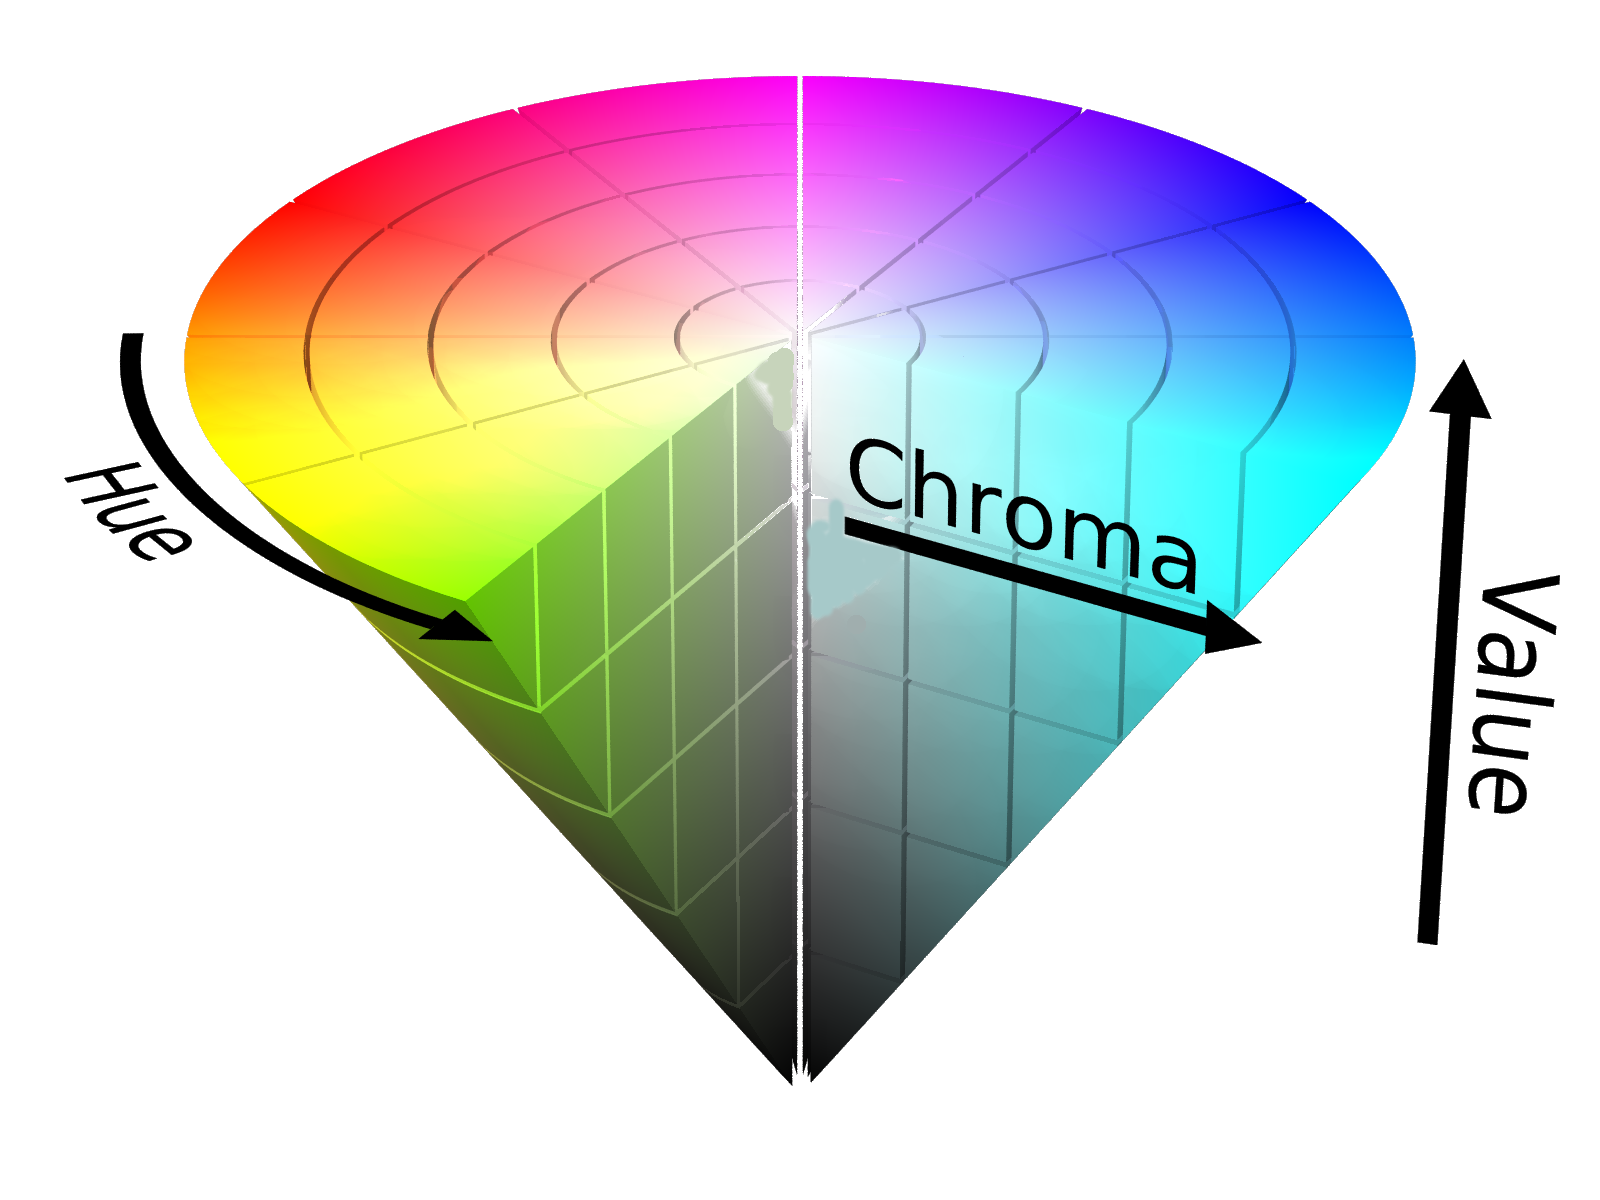
\includegraphics[scale=0.2]{img/HSV_pyramid.png}
    \caption{Pyramid representation of the HSV channels}
    \label{fig:hsv_pyramid}
\end{figure}


\subsection{Color moments}

\subsection{The first two moments}

For a discrete random variable $X$, the first two moments are defined as:
\begin{itemize}
    \item \textbf{Expected value}: $$\E \left[ X \right] = \mu = \sum_{i = 1}^{n} p_i x_i $$
    \item \textbf{Variance}:  $$ \Var (X)= \E \left[ (X - \E \left[ X \right] )^2 \right] =\sum _{i=1}^{n} p_i (x_{i} - \mu )^{2} $$
\end{itemize}

\subsection{Hu moments}

\subsubsection{Raw moments}

For a two-dimensional continuous function f(x,y) the moment (sometimes called \enquote{raw moment}) of (p + q)th order is defined as: 
$$ M_{pq}=\int \limits _{-\infty }^{\infty }\int \limits _{-\infty }^{\infty }x^{p}y^{q}f(x,y) dx dy $$
for $p$ and $q \in \N $.

\subsubsection{Central moments}

And the central moments are :
$$\mu_{pq}=\int \limits_{-\infty }^{\infty }\int \limits _{-\infty}^{\infty} (x- \bar{x})^{p}(y - \bar{y})^{q} f(x,y) dx dy $$
with $\bar{x}=\frac{M_{10}}{M_{00}}$ and $\bar{y}=\frac{M_{01}}{M_{00}}$

\subsubsection{Normalized central moments}

The normalized central moments are:
$$ \eta_{ij}=\frac{\mu _{ij}}{\mu_{00}^{\gamma}} $$
where $\gamma = 1 + \frac{I + j}{2}$ for $i + j \geq 2$.

\subsubsection{Definition of the Hu moments}

On the base of those Moments, Hu in \cite{Hu1962} introduced 7 Moments which are invariant for translation, rotation and resizing:
\begin{align*}
    I_{1} = & \eta _{20}+\eta _{02} \\
    I_{2} = & (\eta _{20}-\eta _{02})^{2}+4\eta _{11}^{2} \\
    I_{3} = & (\eta _{30}-3\eta _{12})^{2}+(3\eta _{21}-\eta _{03})^{2} \\
    I_{4} = & (\eta _{30}+\eta _{12})^{2}+(\eta _{21}+\eta _{03})^{2} \\
    \begin{split}
        I_{5} = & (\eta _{30}-3\eta _{12})(\eta _{30}+\eta _{12})[(\eta _{30}+\eta _{12})^{2}-3(\eta _{21}+\eta _{03})^{2}] \\
        & +(3\eta _{21}-\eta _{03})(\eta _{21}+\eta _{03})[3(\eta _{30}+\eta _{12})^{2} -(\eta _{21}+\eta _{03})^{2}]
    \end{split} \\
    I_{6} = & (\eta _{20}-\eta _{02})[(\eta _{30}+\eta _{12})^{2}-(\eta _{21}+\eta _{03})^{2}]+4\eta _{11}(\eta _{30}+\eta _{12})(\eta _{21}+\eta _{03}) \\
    \begin{split}
        I_{7} = & (3\eta _{21}-\eta _{03})(\eta _{30}+\eta _{12})[(\eta _{30}+\eta _{12})^{2}-3(\eta _{21}+\eta _{03})^{2}] \\
        & - (\eta _{30}-3\eta _{12})(\eta _{21}+\eta _{03})[3(\eta _{30}+\eta _{12})^{2}-(\eta _{21}+\eta _{03})^{2}]
    \end{split} \\
\end{align*}

\section{Bag-of-Words}
\subsection{Process}

\textbf{Bag-of-Words} \textit{BoW}, also called Bag of features, is a feature descriptor method inspired by information retrieval from textual documents.

As illustrated in Fig. \ref{fig:bow_process}, the main steps are:
\begin{itemize}
    \item detecting keypoints on each picture. In my case, I use a dense grid of evenly spaced points at a fixed scale and orientation.
    \item describing each keypoints, i.e. extract a feature vector on a neighbourhood of pixels. SIFT, HOG and SURF are common descriptors.
    \item Generating a fix number of visual words that compose our codebook.
    \item We express each image as an histogram of these words' appearance.
\end{itemize}

The combination of a dense grid and SIFT is commonly called dense SIFT. It has been showed to have greater accuracy than using SIFT for keypoint detection and description.

\begin{figure}
    \centering
    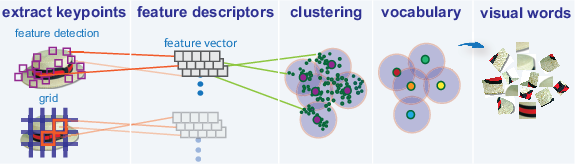
\includegraphics[scale=0.9]{img/bow.png}
    \caption{Illustration of the Bag-Of-Visual-Words model}
    \label{fig:bow_process}
\end{figure}

\subsection{SIFT and SURF}

\textbf{Scale-Invariant Feature Transform} \textit{SIFT} is an algorithm used for detection and description of local feature \cite{Lowe2004}.

The major stages of the algorithm are:
\begin{enumerate}
    \item Scale-space extrema detection: The scale space of an image $L(x, y, \sigma)$ is defined as the product of the convolution of a Gaussian filter $G(x, y, \sigma)$ and an image $I(x, y)$:
    $$
    L(x, y, \sigma) = G(x, y, \sigma) * I(x, y)
    $$
    where $*$ is the convolution at $(x, y)$ and $G(x, y, \sigma) = \frac{1}{2 \pi \sigma^2} \exp(-(x^2 + y^2) / 2 \sigma^2)$.
    
    Laplacian of Gaussian $\sigma^2 \nabla^2 G$ produced the most stable image features but are expensive to compute, thus it is approximated as an Difference of Gaussian (scale-normalized LoG for scale-invariance)
    $$
    G(x, y, k \sigma) - G(x, y, \sigma) \approx (k - 1) \sigma^2 \nabla^2 G
    $$
    
    As presented in figure \ref{fig:sift_difference_of_gaussian}, pyramid of DoG for each octave of scale space is computed: the initial image is repeatedly convolved with Gaussian filters for different values of $\sigma$ to produce the set of scale space images shown on the left. Adjacent Gaussian images are subtracted to produce the difference-of-Gaussian.
    
    \begin{figure}[h]
        \centering
        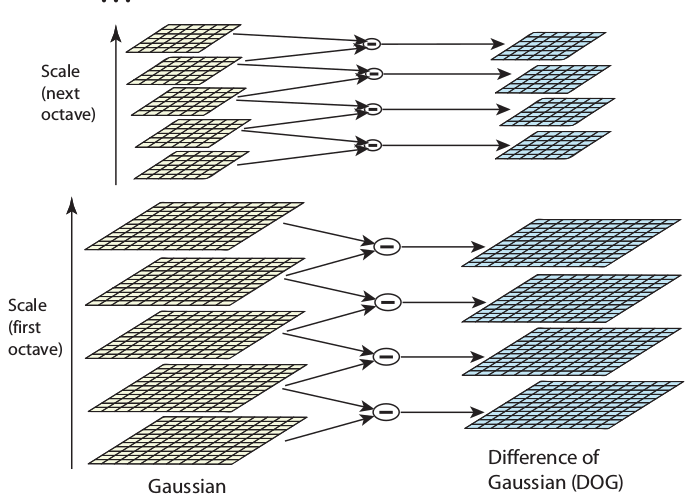
\includegraphics[scale=0.5]{img/sift_difference_of_gaussian.png}
        \caption{Illustration of the difference of Gaussian over multiple octave}
        \label{fig:sift_difference_of_gaussian}
    \end{figure}
    
    \item Keypoint localisation: In order to detect the local maxima and minima of $D(x, y,\sigma)$, each sample point is compared to its eight neighbours in the current image and nine neighbours in the scale above and below. Low contrast and edge keypoints are filtered.
    
    \item Orientation and magnitude assignment: by assigning a consistent orientation to each keypoint based on local image properties, the keypoint descriptor can be represented relative to this orientation and therefore achieve invariance to image rotation.
    
    The magnitude and orientation are defined as:
    $$
    m(x, y) = \sqrt{ \left( L(x +1, y) - L(x -1, y)  \right)^2 + \left( L(x, y + 1) - L(x, y - 1) \right)^2}
    $$
    $$
    \theta(x, y) =\tan^{-1} ( \frac{L(x, y + 1) - L(x, y - 1 )}{L(x + 1, y) - L(x - 1, y)} )
    $$
    
    \item Keypoint descriptor: the local image gradients of a keypoint as presented in figure \ref{fig:sift_descriptor} are computed and accumulated in a histogram. An additional Gaussian weighting function is applied to give less importance to gradients farther away from the keypoint centrer. Once a keypoint candidate has been found by comparing a pixel to its neighbours, the next step is to perform a detailed fit to the nearby data for location, scale, and ratio of principal curvatures. This information allows points to be rejected that have low contrast (and are therefore sensitive to noise) or are poorly localized along an edge.
    
    Usually, SIFT is evaluated at 8 orientation planes over a 4 × 4 neighbourhood giving a
    128-dimension feature vector
    
    \begin{figure}[h]
        \centering
        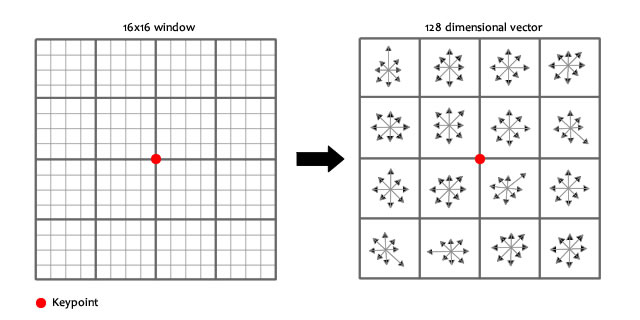
\includegraphics[scale=0.5]{img/sift_descriptor.jpg}
        \caption{Illustration of SIFT as a local image descriptor}
        \label{fig:sift_descriptor}
    \end{figure}
\end{enumerate}

As proven in \cite{Lowe2004}, this method is invariant to translation, scaling and rotation of the picture and is robust to illumination changes, addition of noise, change in the 3-D viewpoint and local geometric distortion.

Multiple variant of SIFT exists. Colour SIFT computes the SIFT in the same manner than the grey scale, except that it does it for each channel independently. Root SIFT is a simple variant of SIFT, presented in \cite{Arandjelovic2012}. When the SIFT descriptors as been computed for each keypoints, we apply an element wise square root of the L1 normalized SIFT vectors


However the SIFT algorithm is quite slow method. That's why in \cite{Bay2006}, the authors present a faster algorithm base on the SIFT approach - \textbf{Speeded Up Robust Features} \textit{SURF}. 
The key is to approximate the LoG with the Box Filter which is the other approximation but of DoG. Using them, the integral image can be constructed and used, which speeds up the whole process since there is no need to iteratively apply those filters one by one (it can be even parallelized). This approach is eagerly applied in the real-time object recognition tasks.

\subsection{K-mean clustering}

Given a set of observations $(x_1, x_2, …, x_n)$, where each observation is a real vector, $k$-means clustering aims to partition the $n$ observations into $k$ $(k \leq n)$ sets $S = {S_1, S_2, …, S_k}$ so as to minimize the within-cluster sum of squares (sum of distance functions of each point in the cluster to its closest centre K). In other words, its objective is to find:

\begin{equation} \label{eq:kmean_objective}
    \underset {S}{\argmin} \sum _{i=1}^{k} \sum _{x \in S_{i}} \left\| x - \mu_{i} \right\|^{2}
\end{equation}

Problem, the exact solution is a NP hard problem. That's why, we can use Lloyd's heuristic algorithm to compute an estimation.

It is an iterative method that find a local minima of the Eq. \ref{eq:kmean_objective}:

\begin{enumerate}
    \item A set of $k$ initial \enquote{means} is chosen randomly within the data domain $M = \{m_1, m_2, \ldots, m_k \}$
    
    \item Then, k clusters are created by associating every observation with the nearest mean.
    $$ \forall i \in \{ 1, \ldots, k \}, ~~ S_{i}^{(t)}= \big \{ x_{p}:{\big \|}x_{p}-m_{i}^{(t)}{\big \|}^{2}\leq {\big \|}x_{p}-m_{j}^{(t)}{\big \|}^{2} ~ \forall j \in \{ 1, \ldots, k \} \big \}$$
    
    \item The centroid of each of the k clusters becomes the new mean.
    $$ \forall i \in \{ 1, \ldots, k \}, ~~ m_{i}^{(t+1)}=\frac {1}{\lvert S_{i}^{(t)} \rvert } \sum _{x_{j} \in S_{i}^{(t)}} x_{j} $$
    
    \item Repeats step 2 and 3 until $M$ not longer changes.
\end{enumerate}

The centroid results and number of iterations are highly dependant of the initial centroid. As a result, the computation is often done several times, with different initialisations.

To help to overcome this issue, the \enquote{kmeans++} initialisation scheme is often used, which has been described in \cite{Arthur2007}. This method initializes the centroids to be (generally) distant from each other, leading to provably better results than random initialization.
